
%% bare_jrnl.tex
%% V1.3
%% 2007/01/11
%% by Michael Shell
%% see http://www.michaelshell.org/
%% for current contact information.
%%
%% This is a skeleton file demonstrating the use of IEEEtran.cls
%% (requires IEEEtran.cls version 1.7 or later) with an IEEE journal paper.
%%
%% Support sites:
%% http://www.michaelshell.org/tex/ieeetran/
%% http://www.ctan.org/tex-archive/macros/latex/contrib/IEEEtran/
%% and
%% http://www.ieee.org/



% *** Authors should verify (and, if needed, correct) their LaTeX system  ***
% *** with the testflow diagnostic prior to trusting their LaTeX platform ***
% *** with production work. IEEE's font choices can trigger bugs that do  ***
% *** not appear when using other class files.                            ***
% The testflow support page is at:
% http://www.michaelshell.org/tex/testflow/


%%*************************************************************************
%% Legal Notice:
%% This code is offered as-is without any warranty either expressed or
%% implied; without even the implied warranty of MERCHANTABILITY or
%% FITNESS FOR A PARTICULAR PURPOSE! 
%% User assumes all risk.
%% In no event shall IEEE or any contributor to this code be liable for
%% any damages or losses, including, but not limited to, incidental,
%% consequential, or any other damages, resulting from the use or misuse
%% of any information contained here.
%%
%% All comments are the opinions of their respective authors and are not
%% necessarily endorsed by the IEEE.
%%
%% This work is distributed under the LaTeX Project Public License (LPPL)
%% ( http://www.latex-project.org/ ) version 1.3, and may be freely used,
%% distributed and modified. A copy of the LPPL, version 1.3, is included
%% in the base LaTeX documentation of all distributions of LaTeX released
%% 2003/12/01 or later.
%% Retain all contribution notices and credits.
%% ** Modified files should be clearly indicated as such, including  **
%% ** renaming them and changing author support contact information. **
%%
%% File list of work: IEEEtran.cls, IEEEtran_HOWTO.pdf, bare_adv.tex,
%%                    bare_conf.tex, bare_jrnl.tex, bare_jrnl_compsoc.tex
%%*************************************************************************

% Note that the a4paper option is mainly intended so that authors in
% countries using A4 can easily print to A4 and see how their papers will
% look in print - the typesetting of the document will not typically be
% affected with changes in paper size (but the bottom and side margins will).
% Use the testflow package mentioned above to verify correct handling of
% both paper sizes by the user's LaTeX system.
%
% Also note that the "draftcls" or "draftclsnofoot", not "draft", option
% should be used if it is desired that the figures are to be displayed in
% draft mode.
%
\documentclass[journal]{IEEEtran}
\usepackage{blindtext}
\usepackage{graphicx}

% Some very useful LaTeX packages include:
% (uncomment the ones you want to load)


% *** MISC UTILITY PACKAGES ***
%
%\usepackage{ifpdf}
% Heiko Oberdiek's ifpdf.sty is very useful if you need conditional
% compilation based on whether the output is pdf or dvi.
% usage:
% \ifpdf
%   % pdf code
% \else
%   % dvi code
% \fi
% The latest version of ifpdf.sty can be obtained from:
% http://www.ctan.org/tex-archive/macros/latex/contrib/oberdiek/
% Also, note that IEEEtran.cls V1.7 and later provides a builtin
% \ifCLASSINFOpdf conditional that works the same way.
% When switching from latex to pdflatex and vice-versa, the compiler may
% have to be run twice to clear warning/error messages.






% *** CITATION PACKAGES ***
%
%\usepackage{cite}
% cite.sty was written by Donald Arseneau
% V1.6 and later of IEEEtran pre-defines the format of the cite.sty package
% \cite{} output to follow that of IEEE. Loading the cite package will
% result in citation numbers being automatically sorted and properly
% "compressed/ranged". e.g., [1], [9], [2], [7], [5], [6] without using
% cite.sty will become [1], [2], [5]--[7], [9] using cite.sty. cite.sty's
% \cite will automatically add leading space, if needed. Use cite.sty's
% noadjust option (cite.sty V3.8 and later) if you want to turn this off.
% cite.sty is already installed on most LaTeX systems. Be sure and use
% version 4.0 (2003-05-27) and later if using hyperref.sty. cite.sty does
% not currently provide for hyperlinked citations.
% The latest version can be obtained at:
% http://www.ctan.org/tex-archive/macros/latex/contrib/cite/
% The documentation is contained in the cite.sty file itself.






% *** GRAPHICS RELATED PACKAGES ***
%
\ifCLASSINFOpdf
  % \usepackage[pdftex]{graphicx}
  % declare the path(s) where your graphic files are
  % \graphicspath{{../pdf/}{../jpeg/}}
  % and their extensions so you won't have to specify these with
  % every instance of \includegraphics
  % \DeclareGraphicsExtensions{.pdf,.jpeg,.png}
\else
  % or other class option (dvipsone, dvipdf, if not using dvips). graphicx
  % will default to the driver specified in the system graphics.cfg if no
  % driver is specified.
  % \usepackage[dvips]{graphicx}
  % declare the path(s) where your graphic files are
  % \graphicspath{{../eps/}}
  % and their extensions so you won't have to specify these with
  % every instance of \includegraphics
  % \DeclareGraphicsExtensions{.eps}
\fi
% graphicx was written by David Carlisle and Sebastian Rahtz. It is
% required if you want graphics, photos, etc. graphicx.sty is already
% installed on most LaTeX systems. The latest version and documentation can
% be obtained at: 
% http://www.ctan.org/tex-archive/macros/latex/required/graphics/
% Another good source of documentation is "Using Imported Graphics in
% LaTeX2e" by Keith Reckdahl which can be found as epslatex.ps or
% epslatex.pdf at: http://www.ctan.org/tex-archive/info/
%
% latex, and pdflatex in dvi mode, support graphics in encapsulated
% postscript (.eps) format. pdflatex in pdf mode supports graphics
% in .pdf, .jpeg, .png and .mps (metapost) formats. Users should ensure
% that all non-photo figures use a vector format (.eps, .pdf, .mps) and
% not a bitmapped formats (.jpeg, .png). IEEE frowns on bitmapped formats
% which can result in "jaggedy"/blurry rendering of lines and letters as
% well as large increases in file sizes.
%
% You can find documentation about the pdfTeX application at:
% http://www.tug.org/applications/pdftex





% *** MATH PACKAGES ***
%
%\usepackage[cmex10]{amsmath}
% A popular package from the American Mathematical Society that provides
% many useful and powerful commands for dealing with mathematics. If using
% it, be sure to load this package with the cmex10 option to ensure that
% only type 1 fonts will utilized at all point sizes. Without this option,
% it is possible that some math symbols, particularly those within
% footnotes, will be rendered in bitmap form which will result in a
% document that can not be IEEE Xplore compliant!
%
% Also, note that the amsmath package sets \interdisplaylinepenalty to 10000
% thus preventing page breaks from occurring within multiline equations. Use:
%\interdisplaylinepenalty=2500
% after loading amsmath to restore such page breaks as IEEEtran.cls normally
% does. amsmath.sty is already installed on most LaTeX systems. The latest
% version and documentation can be obtained at:
% http://www.ctan.org/tex-archive/macros/latex/required/amslatex/math/





% *** SPECIALIZED LIST PACKAGES ***
%
%\usepackage{algorithmic}
% algorithmic.sty was written by Peter Williams and Rogerio Brito.
% This package provides an algorithmic environment fo describing algorithms.
% You can use the algorithmic environment in-text or within a figure
% environment to provide for a floating algorithm. Do NOT use the algorithm
% floating environment provided by algorithm.sty (by the same authors) or
% algorithm2e.sty (by Christophe Fiorio) as IEEE does not use dedicated
% algorithm float types and packages that provide these will not provide
% correct IEEE style captions. The latest version and documentation of
% algorithmic.sty can be obtained at:
% http://www.ctan.org/tex-archive/macros/latex/contrib/algorithms/
% There is also a support site at:
% http://algorithms.berlios.de/index.html
% Also of interest may be the (relatively newer and more customizable)
% algorithmicx.sty package by Szasz Janos:
% http://www.ctan.org/tex-archive/macros/latex/contrib/algorithmicx/




% *** ALIGNMENT PACKAGES ***
%
%\usepackage{array}
% Frank Mittelbach's and David Carlisle's array.sty patches and improves
% the standard LaTeX2e array and tabular environments to provide better
% appearance and additional user controls. As the default LaTeX2e table
% generation code is lacking to the point of almost being broken with
% respect to the quality of the end results, all users are strongly
% advised to use an enhanced (at the very least that provided by array.sty)
% set of table tools. array.sty is already installed on most systems. The
% latest version and documentation can be obtained at:
% http://www.ctan.org/tex-archive/macros/latex/required/tools/


%\usepackage{mdwmath}
%\usepackage{mdwtab}
% Also highly recommended is Mark Wooding's extremely powerful MDW tools,
% especially mdwmath.sty and mdwtab.sty which are used to format equations
% and tables, respectively. The MDWtools set is already installed on most
% LaTeX systems. The lastest version and documentation is available at:
% http://www.ctan.org/tex-archive/macros/latex/contrib/mdwtools/


% IEEEtran contains the IEEEeqnarray family of commands that can be used to
% generate multiline equations as well as matrices, tables, etc., of high
% quality.


%\usepackage{eqparbox}
% Also of notable interest is Scott Pakin's eqparbox package for creating
% (automatically sized) equal width boxes - aka "natural width parboxes".
% Available at:
% http://www.ctan.org/tex-archive/macros/latex/contrib/eqparbox/





% *** SUBFIGURE PACKAGES ***
\usepackage[tight,footnotesize]{subfigure}
% subfigure.sty was written by Steven Douglas Cochran. This package makes it
% easy to put subfigures in your figures. e.g., "Figure 1a and 1b". For IEEE
% work, it is a good idea to load it with the tight package option to reduce
% the amount of white space around the subfigures. subfigure.sty is already
% installed on most LaTeX systems. The latest version and documentation can
% be obtained at:
% http://www.ctan.org/tex-archive/obsolete/macros/latex/contrib/subfigure/
% subfigure.sty has been superceeded by subfig.sty.



%\usepackage[caption=false]{caption}
%\usepackage[font=footnotesize]{subfig}
% subfig.sty, also written by Steven Douglas Cochran, is the modern
% replacement for subfigure.sty. However, subfig.sty requires and
% automatically loads Axel Sommerfeldt's caption.sty which will override
% IEEEtran.cls handling of captions and this will result in nonIEEE style
% figure/table captions. To prevent this problem, be sure and preload
% caption.sty with its "caption=false" package option. This is will preserve
% IEEEtran.cls handing of captions. Version 1.3 (2005/06/28) and later 
% (recommended due to many improvements over 1.2) of subfig.sty supports
% the caption=false option directly:
%\usepackage[caption=false,font=footnotesize]{subfig}
%
% The latest version and documentation can be obtained at:
% http://www.ctan.org/tex-archive/macros/latex/contrib/subfig/
% The latest version and documentation of caption.sty can be obtained at:
% http://www.ctan.org/tex-archive/macros/latex/contrib/caption/




% *** FLOAT PACKAGES ***
%
\usepackage{fixltx2e}
% fixltx2e, the successor to the earlier fix2col.sty, was written by
% Frank Mittelbach and David Carlisle. This package corrects a few problems
% in the LaTeX2e kernel, the most notable of which is that in current
% LaTeX2e releases, the ordering of single and double column floats is not
% guaranteed to be preserved. Thus, an unpatched LaTeX2e can allow a
% single column figure to be placed prior to an earlier double column
% figure. The latest version and documentation can be found at:
% http://www.ctan.org/tex-archive/macros/latex/base/



%\usepackage{stfloats}
% stfloats.sty was written by Sigitas Tolusis. This package gives LaTeX2e
% the ability to do double column floats at the bottom of the page as well
% as the top. (e.g., "\begin{figure*}[!b]" is not normally possible in
% LaTeX2e). It also provides a command:
%\fnbelowfloat
% to enable the placement of footnotes below bottom floats (the standard
% LaTeX2e kernel puts them above bottom floats). This is an invasive package
% which rewrites many portions of the LaTeX2e float routines. It may not work
% with other packages that modify the LaTeX2e float routines. The latest
% version and documentation can be obtained at:
% http://www.ctan.org/tex-archive/macros/latex/contrib/sttools/
% Documentation is contained in the stfloats.sty comments as well as in the
% presfull.pdf file. Do not use the stfloats baselinefloat ability as IEEE
% does not allow \baselineskip to stretch. Authors submitting work to the
% IEEE should note that IEEE rarely uses double column equations and
% that authors should try to avoid such use. Do not be tempted to use the
% cuted.sty or midfloat.sty packages (also by Sigitas Tolusis) as IEEE does
% not format its papers in such ways.


%\ifCLASSOPTIONcaptionsoff
%  \usepackage[nomarkers]{endfloat}
% \let\MYoriglatexcaption\caption
% \renewcommand{\caption}[2][\relax]{\MYoriglatexcaption[#2]{#2}}
%\fi
% endfloat.sty was written by James Darrell McCauley and Jeff Goldberg.
% This package may be useful when used in conjunction with IEEEtran.cls'
% captionsoff option. Some IEEE journals/societies require that submissions
% have lists of figures/tables at the end of the paper and that
% figures/tables without any captions are placed on a page by themselves at
% the end of the document. If needed, the draftcls IEEEtran class option or
% \CLASSINPUTbaselinestretch interface can be used to increase the line
% spacing as well. Be sure and use the nomarkers option of endfloat to
% prevent endfloat from "marking" where the figures would have been placed
% in the text. The two hack lines of code above are a slight modification of
% that suggested by in the endfloat docs (section 8.3.1) to ensure that
% the full captions always appear in the list of figures/tables - even if
% the user used the short optional argument of \caption[]{}.
% IEEE papers do not typically make use of \caption[]'s optional argument,
% so this should not be an issue. A similar trick can be used to disable
% captions of packages such as subfig.sty that lack options to turn off
% the subcaptions:
% For subfig.sty:
% \let\MYorigsubfloat\subfloat
% \renewcommand{\subfloat}[2][\relax]{\MYorigsubfloat[]{#2}}
% For subfigure.sty:
% \let\MYorigsubfigure\subfigure
% \renewcommand{\subfigure}[2][\relax]{\MYorigsubfigure[]{#2}}
% However, the above trick will not work if both optional arguments of
% the \subfloat/subfig command are used. Furthermore, there needs to be a
% description of each subfigure *somewhere* and endfloat does not add
% subfigure captions to its list of figures. Thus, the best approach is to
% avoid the use of subfigure captions (many IEEE journals avoid them anyway)
% and instead reference/explain all the subfigures within the main caption.
% The latest version of endfloat.sty and its documentation can obtained at:
% http://www.ctan.org/tex-archive/macros/latex/contrib/endfloat/
%
% The IEEEtran \ifCLASSOPTIONcaptionsoff conditional can also be used
% later in the document, say, to conditionally put the References on a 
% page by themselves.





% *** PDF, URL AND HYPERLINK PACKAGES ***
%
%\usepackage{url}
% url.sty was written by Donald Arseneau. It provides better support for
% handling and breaking URLs. url.sty is already installed on most LaTeX
% systems. The latest version can be obtained at:
% http://www.ctan.org/tex-archive/macros/latex/contrib/misc/
% Read the url.sty source comments for usage information. Basically,
% \url{my_url_here}.





% *** Do not adjust lengths that control margins, column widths, etc. ***
% *** Do not use packages that alter fonts (such as pslatex).         ***
% There should be no need to do such things with IEEEtran.cls V1.6 and later.
% (Unless specifically asked to do so by the journal or conference you plan
% to submit to, of course. )


% correct bad hyphenation here
\hyphenation{op-tical net-works semi-conduc-tor}

%Change captions
\usepackage{subcaption}
\usepackage[font=footnotesize,labelfont=normalfont ]{caption}
\captionsetup[table]{name=Table,belowskip=3pt,aboveskip=4pt}
\renewcommand{\thetable}{\arabic{table}}

%Allow for pbox formatting in table
\usepackage{pbox}
\usepackage{array}
\usepackage{subcaption}
\usepackage{amsmath}

\begin{document}
%

% paper title
% can use linebreaks \\ within to get better formatting as desired
\title{Predicting the Number of Students, grades K-5, in NYC at the Census Tract Level}
%
%
% author names and IEEE memberships
% note positions of commas and nonbreaking spaces ( ~ ) LaTeX will not break
% a structure at a ~ so this keeps an author's name from being broken across
% two lines.
% use \thanks{} to gain access to the first footnote area
% a separate \thanks must be used for each paragraph as LaTeX2e's \thanks
% was not built to handle multiple paragraphs
%

\author{Ben~Jakubowski~and~Michael~Higgins}

% note the % following the last \IEEEmembership and also \thanks - 
% these prevent an unwanted space from occurring between the last author name
% and the end of the author line. i.e., if you had this:
% 
% \author{....lastname \thanks{...} \thanks{...} }
%                     ^------------^------------^----Do not want these spaces!
%
% a space would be appended to the last name and could cause every name on that
% line to be shifted left slightly. This is one of those "LaTeX things". For
% instance, "\textbf{A} \textbf{B}" will typeset as "A B" not "AB". To get
% "AB" then you have to do: "\textbf{A}\textbf{B}"
% \thanks is no different in this regard, so shield the last } of each \thanks
% that ends a line with a % and do not let a space in before the next \thanks.
% Spaces after \IEEEmembership other than the last one are OK (and needed) as
% you are supposed to have spaces between the names. For what it is worth,
% this is a minor point as most people would not even notice if the said evil
% space somehow managed to creep in.



% The paper headers
\markboth{NYU INFERENCE AND REPRESENTATION PROJECT 2016}%
{Shell \MakeLowercase{\textit{et al.}}: Bare Demo of IEEEtran.cls for Journals}
% The only time the second header will appear is for the odd numbered pages
% after the title page when using the twoside option.
% 
% *** Note that you probably will NOT want to include the author's ***
% *** name in the headers of peer review papers.                   ***
% You can use \ifCLASSOPTIONpeerreview for conditional compilation here if
% you desire.




% If you want to put a publisher's ID mark on the page you can do it like
% this:
%\IEEEpubid{0000--0000/00\$00.00~\copyright~2007 IEEE}
% Remember, if you use this you must call \IEEEpubidadjcol in the second
% column for its text to clear the IEEEpubid mark.



% use for special paper notices
%\IEEEspecialpapernotice{(Invited Paper)}




% make the title area
\maketitle


\begin{abstract}
%\boldmath
In 2016, the NYC Department of Education released a Call for Innovations requesting submission of predictive models that gave MSE-minimizing predictions of the number of students in each grade K-5, for each census tract in  School District 20, for each year from 2011-12 to 2015-2016. We report on development of two types of probabilistic graphical models developed for this predictive task. Both models are premised on the hypothesis that priors which induce spatial smoothness could help reduce overfitting and yield better predictive models. Unfortunately, this core hypothesis was not supported by our experiments. Regardless, we report our results, provide potential explanations, and suggest alternative approaches.
\end{abstract}
% IEEEtran.cls defaults to using nonbold math in the Abstract.
% This preserves the distinction between vectors and scalars. However,
% if the journal you are submitting to favors bold math in the abstract,
% then you can use LaTeX's standard command \boldmath at the very start
% of the abstract to achieve this. Many IEEE journals frown on math
% in the abstract anyway.

% Note that keywords are not normally used for peerreview papers.
\begin{IEEEkeywords}
Areal spatiotemporal data, Gaussian Markov Random Fields, Stan
\end{IEEEkeywords}






% For peer review papers, you can put extra information on the cover
% page as needed:
% \ifCLASSOPTIONpeerreview
% \begin{center} \bfseries EDICS Category: 3-BBND \end{center}
% \fi
%
% For peerreview papers, this IEEEtran command inserts a page break and
% creates the second title. It will be ignored for other modes.
\IEEEpeerreviewmaketitle



\section{Introduction}

In the fall of 2016, the New York City (NYC) Department of Education (DoE) released a Call for Innovations, or public call for submissions addressing a pressing civic need. The DoE specifically was soliciting proposals for "Enhancing School Zoning Efforts by Predicting Population Change." Since the DoE serves over 1.1 million students, they were interested in more accurately projecting population changes in order to inform school zoning and resource allocation decisions.

Their Call for Innovations was divided into multiple stages; we developed a submission for the initial modeling stage as our project for the NYU class Inference and Representation. Specifically, in this initial modelling stage of the challenge, teams were asked to develop predictive models for the following predictive task:
\begin{itemize}
\item For each census tract $k$ in NYC School District 20 (142 tracts):
\begin{itemize}
\item For each grade $g$ in K-5:
\begin{itemize}
\item Using data from the school years 2001-2002 to 2010-2011, for each year $t$ from 2010-2011 to 2014-2015:
\begin{itemize}
\item \textbf{Target}: Predict the total number of students in grade $g$ in tract $k$ enrolled in public or charter schools in year $t$.
\end{itemize}
\end{itemize}
\end{itemize}
\end{itemize}
An accurate predictive model for this task would help the DoE better plan for and serve the evolving needs of NYC families. Unfortunately, this problem is very difficult because it requires making a large number of predictions given a small amount of training data.  For each tract, only 10 years of counts are available for each grade, and these 10 years of data are being used to support 5 years of projections.

Given this problem structure (making a large number of predictions using a very small data set), we decided to test models that allow for sharing of information across tracts. Specifically, we hypothesized that gains could be made by exploiting the spatial structure of the data: if counts for adjacent census tracts are similar, then models that capture neighborhood structure would be more robust than independently modeling each tract.

In addition to exploring models that capture this hypothesized spatial structure, we also chose to constrain our models by not consuming side data. This choice reflected the following deployment constraints and hypotheses:
\begin{itemize}
\item \textbf{Constraint}: Since the model is intended to project counts for five years, we would need to restrict the allowed feature set to features available prior to the prediction window.
\item \textbf{Hypothesis} Additionally, in the second modeling stage for this contest, predictions are supposed to be made at the city block level. We assumed the following: given the numbers of students in grades K-5 for 10 past years, no readily available city-block level features (available prior to the five year prediction window) would provide additional information regarding the targets.
\end{itemize}
Based on these hypotheses and constraints, we tested the performance of two types of models:
\begin{enumerate}
    \item Spatially correlated linear models.
    \item Spatially correlated markov chain models.
\end{enumerate}
Results and analysis for each of these models is presented in the subsequent sections.

\section{Related Work}

Our models are all inspired by the areal spatiotemporal models presented by Lee, Rushworth, and Napier in the vignette for their R package \texttt{CARBayesST} \cite{lee2015carbayesst}. In this package\footnote{As a side note, in the course of this project the authors identified a bug in their implementation of the log likelihood extractor, and were able to contribute to this package by reporting it to Lee.}, Lee \emph{et al} developed Gibbs samplers for a number of spatiotemporal mixed effects models, including a temporally linear, spatially correlated model. Letting $t$ be time, temporal linearity is apparent from the first component of the model specification (which, using the semantics of the applied statistics community, is simply a hierarchical, or random effects, model for a single district):
\begin{align*}
    &\textrm{Target in spatial unit }k\textrm{ at time }t:\\
    &~~~~Y_{kt}\sim \textrm{N}(x_{kt}^T\beta + \phi_{kt},\nu^2)\\
    &\textrm{Latent spatiotemporal variable:}\\
    &~~~~\phi_{kt} = \underbrace{\beta_1}_{\substack{\textrm{District}\\\textrm{intercept}}} + \overbrace{\phi_k}^{\substack{\textrm{Tract}\\\textrm{intercept}}}~+~(\underbrace{\alpha}_{\substack{\textrm{District}\\\textrm{slope}}}+ \overbrace{\delta_k}^{\substack{\textrm{Tract}\\\textrm{slope}}})\frac{(t - \bar{t})}{N}
\end{align*}
While the first component of the model specification implies temporal linearity, it does not impose spatial smoothness on the random effects. This is achieved through the priors placed on $\phi_{k}$ and $\delta_{k}$. Described by Lee \emph{et al} as conditional autoregressive (CAR) priors, they are simply Gaussian Markov Random Fields (GMRFs) (as shown in Fig. \ref{fig:MRF}) where the graph structure maps onto the spatial units' neighborhood structure.

\begin{figure}[!h]
    \centering
    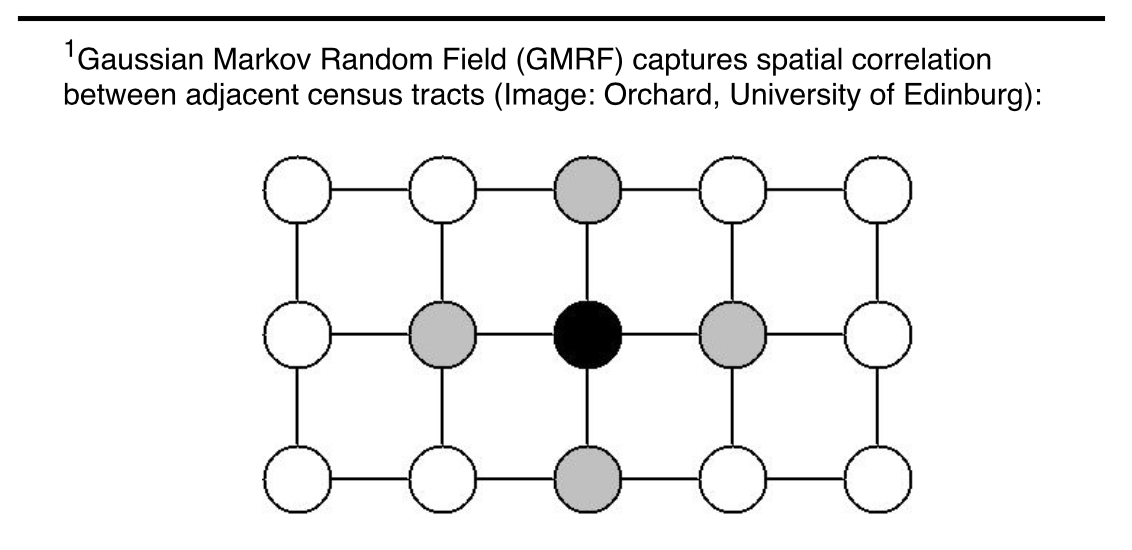
\includegraphics[width=3in,height=2.5in,clip,keepaspectratio]{MRF.png}
    \caption{General structure of a Markov Field on a lattice}
    \label{fig:MRF}
\end{figure}

The form of the GMRF prior described by Lee \emph{et al} was first proposed by Besag \emph{et al} \cite{besag1991bayesian} for use in image restoration (where pixels have a natural neighborhood structure), and then modified by Leroux \emph{et al} \cite{leroux2000estimation} to allow for varying strength of the spatial relationship.

Specifically, given the adjacency matrix $W$ for the spatial units, the conditional priors are given by:
\begin{align*}
    & \phi_k | \boldmath{\phi}_{-k}, \boldmath{W}  ~ \sim \\
    &~~\textrm{N}\left(\frac{\rho_{int}\sum_{j = 1}^K w_{kj}\phi_j}{\rho_{int}\sum_{j = 1}^K w_{kj} + 1 - \rho_{int}}, \frac{\tau_{int}^2}{\rho_{int}\sum_{j = 1}^K w_{kj} + 1 - \rho_{int}}\right) \\ 
    &~\\
    &\delta_k | \boldmath{\delta}_{-k}, \boldmath{W}  ~ \sim\\
    &~~\textrm{N}\left(\frac{\rho_{slo}\sum_{j = 1}^K w_{kj}\delta_j}{\rho_{slo}\sum_{j = 1}^K w_{kj} + 1 - \rho_{slo}}, \frac{\tau_{slo}^2}{\rho_{slo}\sum_{j = 1}^K w_{kj} + 1 - \rho_{slo}}\right)
\end{align*}

Note these priors are parametrized by two additional parameters: $\rho$, which ranges from [0,1] and controls the strength of the spatial relationship, and $\tau^2$, which controls the variance of the latent spatiotemporal effects. Finally, Lee \emph{et al} state they use weakly informative priors on these parameters:
\begin{align*}
    \tau_{int}^2, \tau_{slo}^2 ~&\sim~ \textrm{Inverse-Gamma}(a,b) \\
    \rho_{int}, \rho_{slo} ~&\sim~ \textrm{Uniform}(0,1)
\end{align*}

While this specifies the model, the structure is perhaps obfuscated by notation. Hence we present Lee \emph{et al}'s model (ignoring hyperpriors and other regression coefficients) in figure \ref{fig:plate_model_1}.

\begin{figure}[h!]
    \centering
    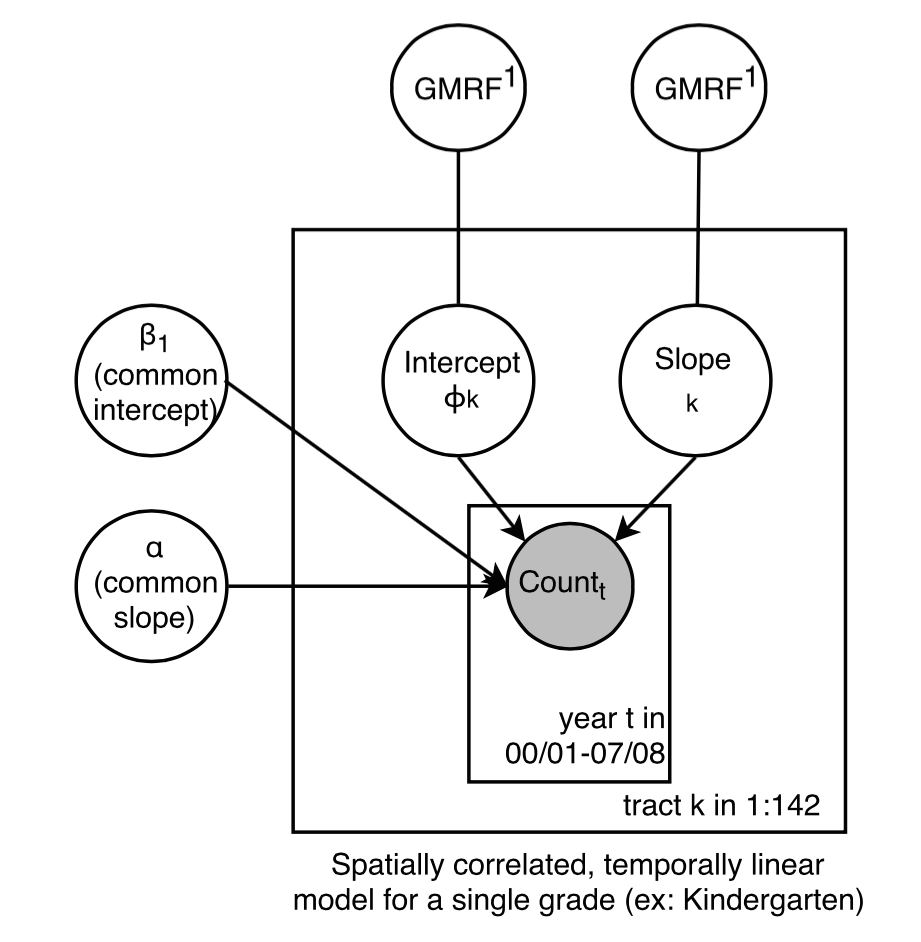
\includegraphics[width=3in,height=2.5in,clip,keepaspectratio]{plate_model_1.png}
    \caption{Graphical model depicting key components of the temporally linear, spatially correlated regression model.}
    \label{fig:plate_model_1}
\end{figure}

This model (and in particular the priors initially proposed by Leroux \cite{leroux2000estimation}) are the basis for our modeling experiments. Importantly, to check our understanding of this model, we first compared the results obtained from (i) using Lee \emph{et al}'s packaged Gibb sampler, and (ii) a from-scratch implemention of the model in Stan, to model counts for a single grade (Kindergarten). These samplers returned similar posterior mean point estimates, providing a sanity check on our from-scratch implemenation (see Fig. \ref{fig:phis_correlation}).

\begin{figure}
    \centering
    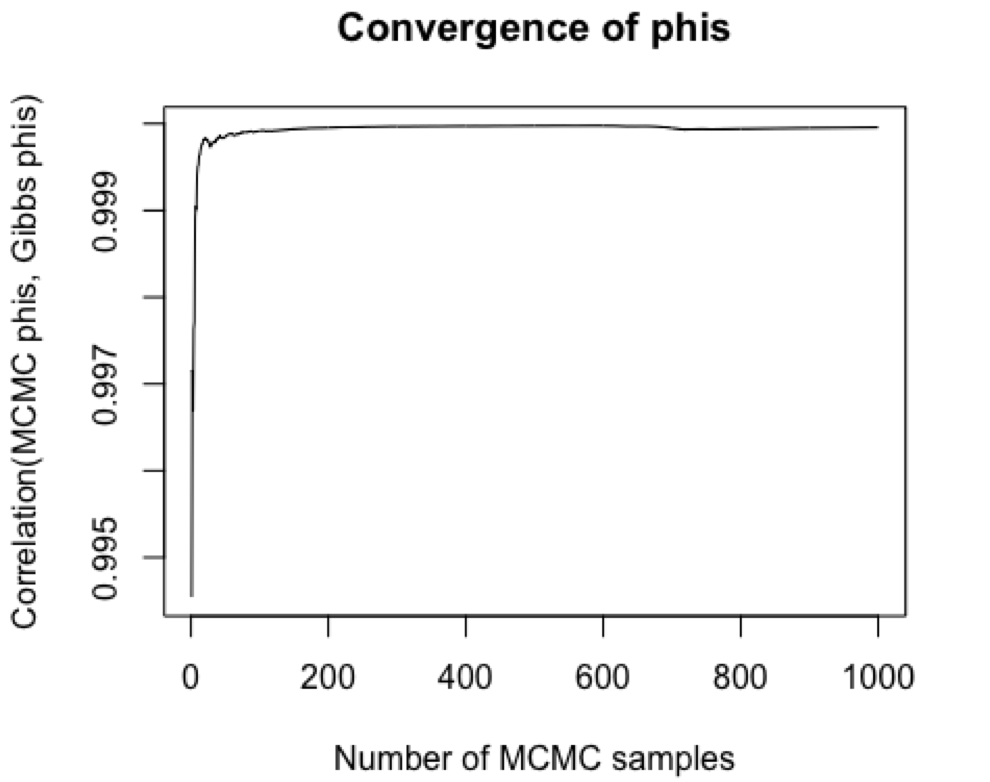
\includegraphics[width=3in,height=2in,clip,keepaspectratio]{convergence_of_phis.png}
    \caption{Correlation between (i) the running posterior mean point estimate of the length-142 \(\boldmath{\phi}\) vector obtained from the Stan model, and (ii) the final posterior mean \(\boldmath{\phi}\) vector obtained after 60,000 samples}
    \label{fig:phis_correlation}
\end{figure}

\section{Problem Definition and Algorithm}
\subsection{Task}
Again, our task is to predict the number of students in grade $g$, year $t$, and census tract $k$ for:
\begin{itemize}
\item $g$ in kindergarden through 5th grade;
\item $t$ in academic years 2011-12 to 2015-16
\item $k$ in set of 142 census tracts in NYC School District 20
\end{itemize}
The available data (for training and testing) are counts for these census tracts and grades, for years from 2001-02 to 2010-2011. Finally, the DoE will be evaluating predictions using mean squared error (MSE) as a loss function.

\subsection{Algorithm}

We approached this predictive task using the following general framework (note detailed information on the specific model families and models is provided in the methodology section):
\begin{enumerate}
    \item We tested two different families of models.
    \item Within each family, we test multiple model variants.
    \item For each specific model, we learned the model (i) with GMRF priors to enforce spatial smoothness, and (ii) without GMRF priors for comparison.
    \item Models were written using the Stan probabilistic programming language \cite{carpenter2016stan}, and the model was fit using  Hamiltonian Markov Chain Monte Carlo sampling.
    \item Training and test set predictions were made using posterior mean point estimates for necessary parameters following sampling.
    \item To evaluate our models we compared the test set MSE performance for (i) the spatially regularized model and (ii) the spatially unregularized model, to determine whether (and to what extent) spatial regularization improved performance.
\end{enumerate}

\section{Experimental Evaluation}
\subsection{Data}

The NYC DoE provided each challenge team with non-zero counts of students, K-5, in each census tract in District 20 in South Brooklyn. Prior to modeling, we followed the following data cleaning procedure:
\begin{enumerate}
    \item We first applied a spatial filter to the provided dataset, only passing records for tracts that were in fact in School District 20. Unfortunately, the provided data included a number of tracts that fell outside of District 20; several weeks into the contest this  was recognized by the DoE and our choice to drop these tracts was validated by the challenge sponsor.
    \item Next, we filled missing values with 0's, since the metadata indicated that missing entries corresponded to an absence of students in that tract for that year.
\end{enumerate}

For greater insight, histograms showing the (smoothed) distributions of counts by grade and year are shown in Fig \ref{fig:hists_grade_year}, and maps showing the counts by grade and year are shown in Fig \ref{fig:maps_grade_year}. Using this data, we proceeded to experiment with two general approaches to modeling, described in the following two modelling sections.

\begin{figure}
\centering
\begin{subfigure}
  \centering
  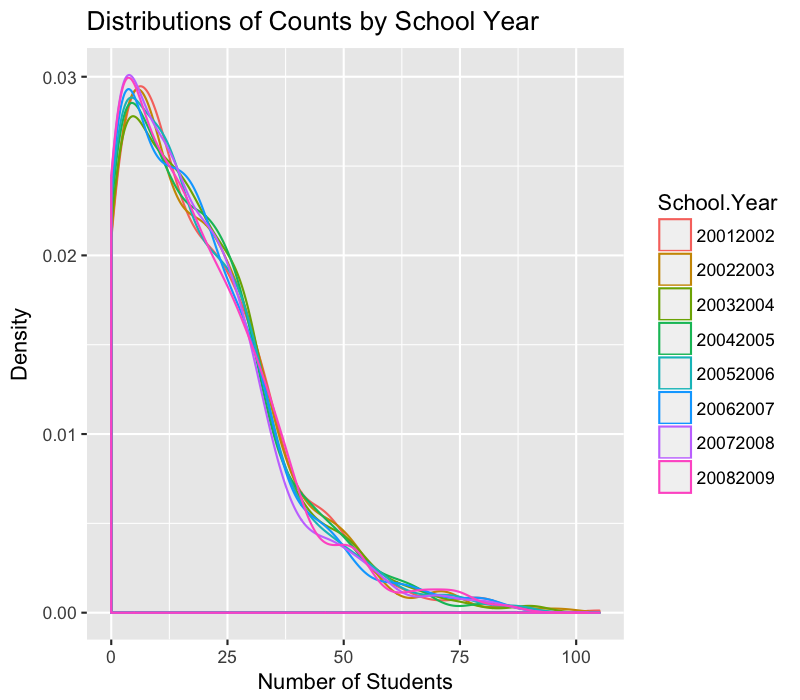
\includegraphics[width=3in,height=2.5in,clip,keepaspectratio]{year_distribution.png}
\end{subfigure}
\begin{subfigure}
  \centering
  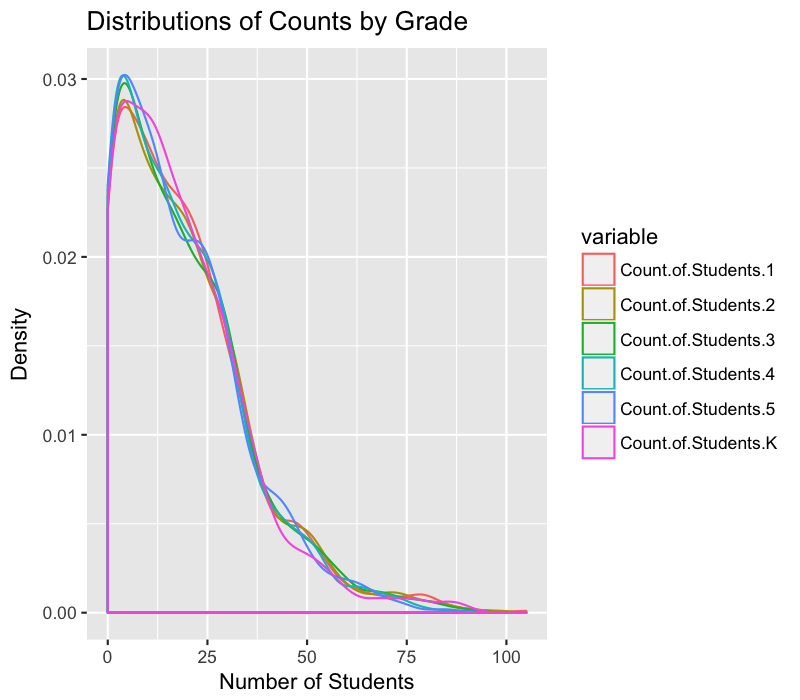
\includegraphics[width=3in,height=2.5in,clip,keepaspectratio]{grade_distribution.png}
\end{subfigure}
\caption{Distributions of counts by year and grade}
\label{fig:hists_grade_year}
\end{figure}

\begin{figure}
\centering
\begin{subfigure}
  \centering
  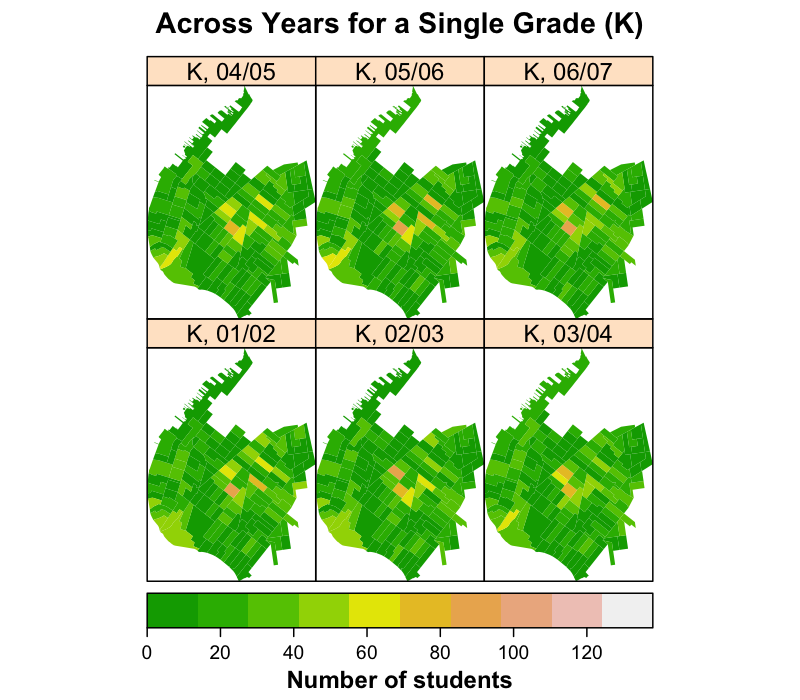
\includegraphics[width=3.5in,height=3.5in,clip,keepaspectratio]{year_map.png}
\end{subfigure}
\begin{subfigure}
  \centering
  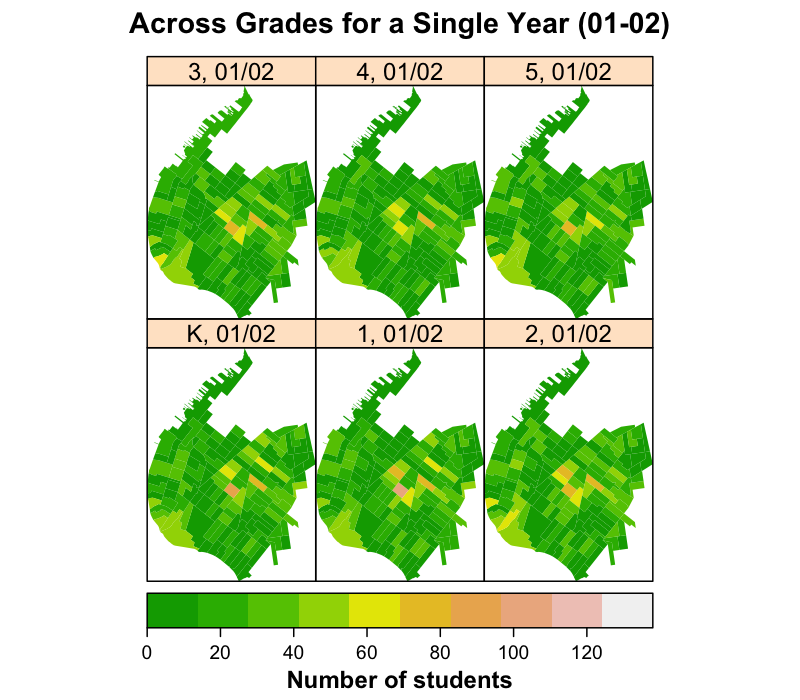
\includegraphics[width=3.5in,height=3.5in,clip,keepaspectratio]{grade_map.png}
\end{subfigure}
\caption{Maps of counts by year and grade}
\label{fig:maps_grade_year}
\end{figure}

\subsection{Model 1: Grade/Time models}

\noindent\emph{Model 1 Methodology} \\

Our first family of models were simply extensions to the spatially correlated linear models presented by Lee \emph{et al}. These models treated grade and year (plus quadratic terms in two models) as covariates in linear models. This is an extension of Lee \emph{et al}'s model, since it introduces additional spatially correlated coeffients (ex: \(\beta_g\)). This model reflects the following hypotheses:
\begin{itemize}
    \item The number of students in a tract $k$ in grade $g$ during year $t$ ($Y_{kgt}$) is well modeled by linear models using features constructed from grade and time.
    \item Moreover, the coefficients in the linear model are drawn from GMRF priors that induce spatial regularization (such that neighboring tracts have similar values for each coefficient).
    \item However, the priors are not shared across coefficients- there are separate priors- since the scales of the effects are hypothesized to vary (i.e. perhaps there is a stronger temporal and a weaker grade effect).
\end{itemize}
While Fig. \ref{fig:plate_model_2} illustrates the general structure of these models, we tested three different versions with increasing complexities:
\begin{enumerate}
    \item  Model 1a: Included $\beta_0, \beta_t, \beta_g$.
    \item  Model 1b (depicted in plate diagram): Included $\beta_0, \beta_t, \beta_g, \beta_{gt}$.
    \item  Model 1c: Included $\beta_0, \beta_t, \beta_g, \beta_{gt}, \beta_{g^2}, \beta_{t^2}$.
\end{enumerate}

\begin{figure}[h!]
    \centering
    \includegraphics[width=3in,height=2in,clip,keepaspectratio]{plate_model_2.png}
    \caption{Example plate diagram for Model 1: spatially correlated linear models. Note we experimented with the three different feature sets.}
    \label{fig:plate_model_2}
\end{figure}

Models were constructed and fit using the Stan probabilistic programming language, using 500 burn-in samples, 1000 samples, and 4 chains. Finally, the posterior mean $\alpha$'s and $\beta$'s across all chains were extracted and used as point estimates for predictive modeling on the test set. \\

\noindent\emph{Model 1 Results} \\

For this model, we used the first 8 years of the provided data as training data, and the last 2 years as test data (as shown in Fig \ref{fig:model_1_train_test}).

\begin{figure}[h!]
    \centering
    \includegraphics[width=3in,height=2.5in,clip,keepaspectratio]{model_1_train_test.png}
    \caption{Training and test sets for Model 1.}
    \label{fig:model_1_train_test}
\end{figure}

For comparison, in addition to learning the model using the CAR/GMRF priors, we also learn equivalent linear models without this spatial regularization. Results from these experiments are provided in Table \ref{tab:model_1_results}.







\begin{table}[h!]
    \centering
    \begin{tabular}{|c|c|c|c|}
        \hline
        Feature set & GMRF prior & Train RMSE & Test RMSE \\
        \hline
        1a: $\beta_0, \beta_t, \beta_g$ & Yes (experimental) & 4.25 & 8.23  \\
        \hline
        1a: $\beta_0, \beta_t, \beta_g$ & No (control) & 4.22 & 8.30  \\
        \hline
        1b: $\beta_0, \beta_t, \beta_g, \beta_{gt}$ & Yes (experimental) & 4.26 & 8.51 \\
        \hline
        1b: $\beta_0, \beta_t, \beta_g, \beta_{gt}$ & No (control) & 4.11 & 8.64 \\
        \hline
        1c: $\beta_0, \beta_t, \beta_g, \beta_{gt}, \beta_{t^2}, \beta_{g^2}$ & Yes (experimental) & 4.25 & 8.29  \\
        \hline
        1c: $\beta_0, \beta_t, \beta_g, \beta_{gt}, \beta_{t^2}, \beta_{g^2}$ & No (control) & 3.98 & 8.55 \\
        \hline
    \end{tabular}
    \caption{Experimental results for Model 1}
    \label{tab:model_1_results}
\end{table}

Based on these results, it is apparent that the CAR prior had a slight regularizing effect on the linear model, especially as the potential for overfitting increased (as more terms were added to models in 1b and 1c). However, they did not significantly improve test set performance.

\subsection{Model 2: Cohort models}

\noindent\emph{Model 2 Methodology} \\

Our second family of models are also extensions of the spatially correlated linear models presented by Lee \emph{et al}, in that they apply the GMRF prior to induce spatial dependence. In Model 1, we treated the grades (rows) and years (columns) as the relevant dimensions of the data matrices, and constructed linear models using (transformations) of these features. In contrast, Model 2 views the diagonals (graduation cohorts) as the relevant observation units.  This model structure is based on the observation that there is less variance within cohorts than within years or grades, as shown in Fig. \ref{fig:directions_of_variance}. This cohort structure is also clear from heatmaps of single census tract data matrices (an example is provided in Fig \ref{fig:heatmap}).

\begin{figure}[h!]
    \centering
    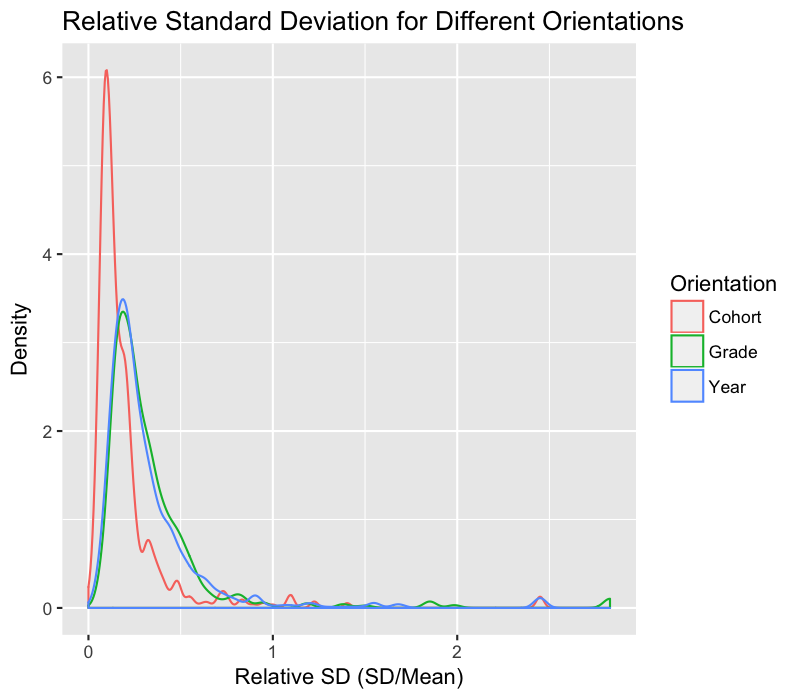
\includegraphics[width=3in,height=2in,clip,keepaspectratio]{directions_of_variance.png}
    \caption{Comparing the relative within grade, year, and cohort relative standard deviations}
    \label{fig:directions_of_variance}
\end{figure}

\begin{figure}
    \centering
    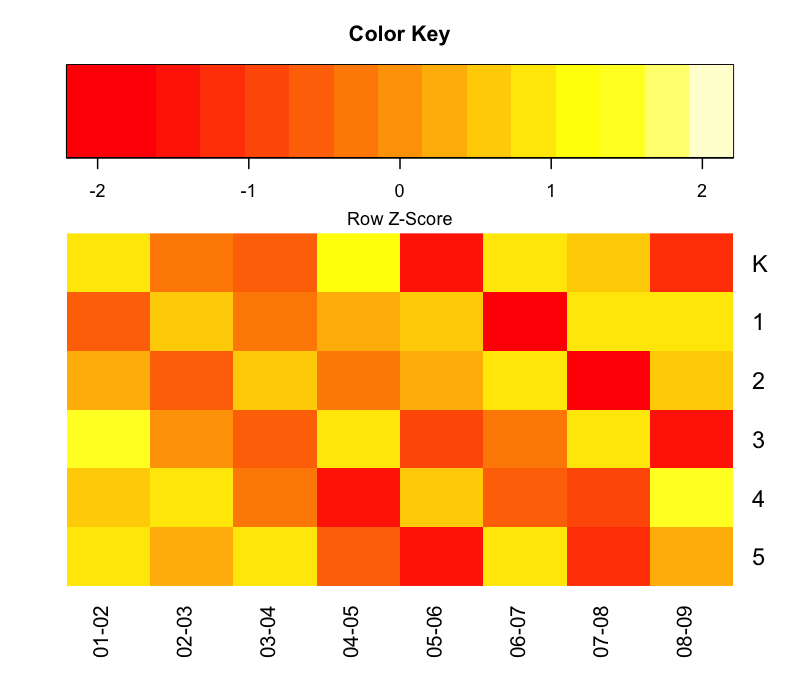
\includegraphics[width=3in,height=2in,clip,keepaspectratio]{heat_map.png}
    \caption{Prediction surface in grade/time/count  space}
    \label{fig:heatmap}
\end{figure}

In addition to viewing cohorts as relevant unit, the model makes a number of strong assumption and operates under strong constraints:
\begin{itemize}
    \item First, the model assumes the student counts form a Markov chain, such that given the most recent observation of cohort size, the cohort evoluation is independent of previous observations.
    \item In addition, the transition operator is parameterized by a single parameter $r_k$, which governs some simple growth process.
    \item Moreover, the parameters in this growth function are drawn from GMRF priors that induce spatial regularization (such that neighboring tracts have similar cohort change behavior).
    \item Finally, this model design suffers from the strong constraint that at least one observation must be made of the cohort size (in grade K-5). As such, it cannot be used to make predictions for the upper triangle in the "projection" section of the matrix depicted in Fig. \ref{fig:cohort_growth}. Hence, it is only useful if it allows for improved prediction in the lower triangle of this matrix and can thus augment a more general model (such as the linear models presented above).
\end{itemize}

Fig. \ref{fig:cohort_growth} illustrates the general structure of these model, with the  counts shaded to represent fully observed training data. Given this general model structure, we tested two different versions of the model:
\begin{enumerate}
    \item  Model 2a encoded linear growth model in the tract-level growth parameter $r_k$, where \(Y_{k(g+1)(t+1)} | Y_{kgt} ~ \sim ~ \textrm{N}(Y_{kgt} + r_k, \nu^2)\).\\
    \item   Model 2b encoded exponential growth in the tract-level growth parameter $r_k$, where \(Y_{k(g+1)(t+1)}|Y_{kgt}  ~ \sim ~ \textrm{N}(Y_{kgt}(1 + r_k), \nu^2)\).
\end{enumerate}

\begin{figure}[h!]
    \centering
    \includegraphics[width=3in,height=2in,clip,keepaspectratio]{cohort_growth.png}
    \caption{Example plate diagram for Model 2: Note we experimented with two different transition operators, both parameterized by a single parameter \(r_k\).}
    \label{fig:cohort_growth}
\end{figure}

Models were constructed and fit using the Stan probabilistic programming language, using 1000 burn-in samples, 5000 samples, and 4 chains. Finally, the posterior mean $r$'s across all chains were extracted and used as point estimates for predictive modeling on the test set. \\

\noindent\emph{Model 2 Results} \\

For this model, we used three cohorts with complete observations as training data to learn \(r\). We then used the remaining data for testing. As shown in Fig \ref{fig:model_2_train_test}, this training/test split allow us to estimate the prediction error for every possible prediction pair (for example projecting the cohort count in grade 5 given grade 1, versus projecting the cohort count in grade 4 given grade 2). 

\begin{figure}[h!]
    \centering
    \includegraphics[width=3in,height=2.5in,clip,keepaspectratio]{model_2_train_test.png}
    \caption{Training and test sets for Model 2.}
    \label{fig:model_2_train_test}
\end{figure}

This is useful since it allows for separate estimation of the error for each potential  prediction. As shown in Fig. \ref{fig:model_2_train_test}, there are five potential predictions made with one-year time steps, four with two-year time steps, three with three-year time steps, two with four-year time steps, and only one with five-year time steps. As such, the error on one-year time steps should be given more weight in the RMSE over the entire prediction space. Finally, for further illustration of this differentiated loss across different prediction tasks, \ref{fig:predict_with_mm} shows the case where we are predicting grades 3, 4, or 5 using grade 2 (i.e. grade 2 is the last observed grade).

\begin{figure}[h!]
    \centering
    \includegraphics[width=3in,height=2.5in,clip,keepaspectratio]{prediction_with_MM.png}
    \caption{Example of prediction using Model 2. Note \[{3_k, 4_k, 5_k} \perp \mathcal{X}\setminus{2_k,r_k} | {r_k, 2_k}\]}
    \label{fig:predict_with_mm}
\end{figure}

Since we are able to get separate prediction RMSE estimates \(\textrm{E}[Y_{k(g+l)(t+l)}~|~Y_{k(g)(t)}]\) for each \(g, l\) pair, we compare the models' performance across all possible pairs. Results are presented as labeled heat-maps in \ref{tab:rmse_for_mm}.

\begin{table}
\begin{tabular}[t]{ m{4cm} m{1cm} }
\centering
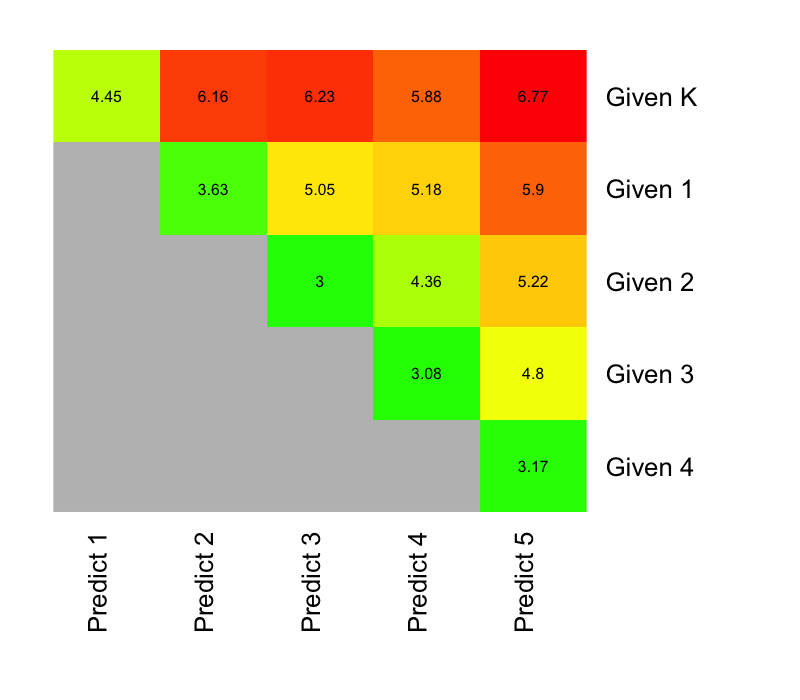
\includegraphics[width=3in,height=1.5in,clip,keepaspectratio]{exp_corr_error.png}
&
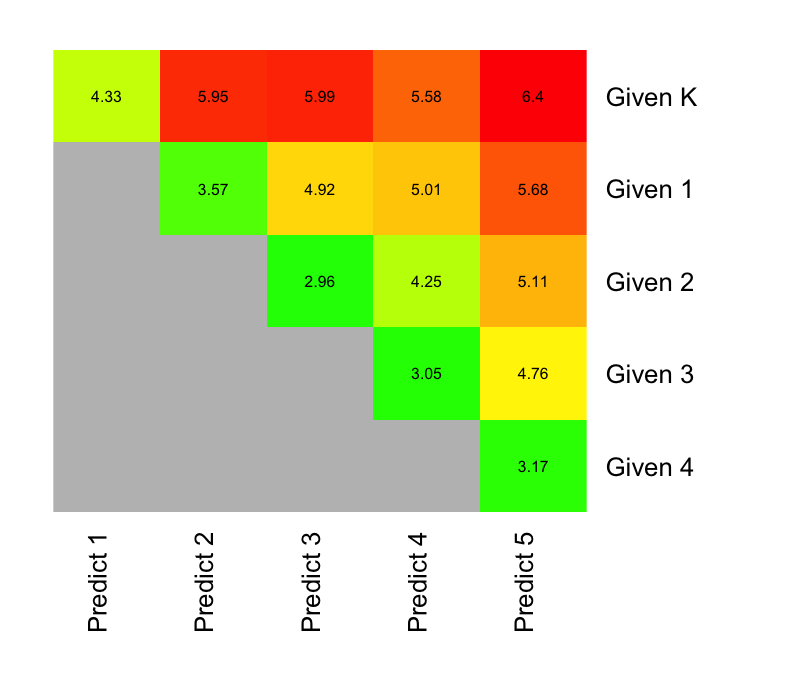
\includegraphics[width=3in,height=1.5in,clip,keepaspectratio]{exp_no_corr_error.png}
\\
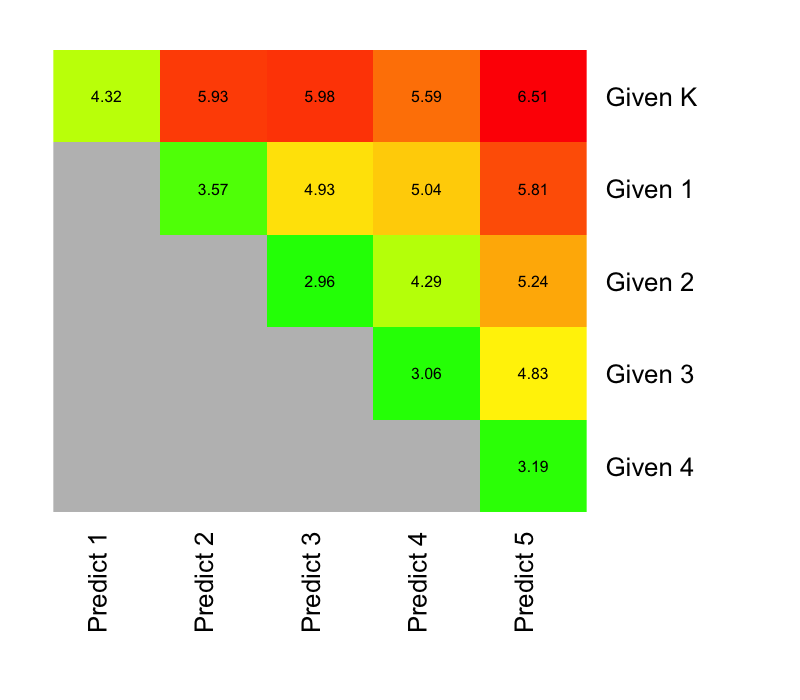
\includegraphics[width=3in,height=1.5in,clip,keepaspectratio]{lin_corr_error.png}
&
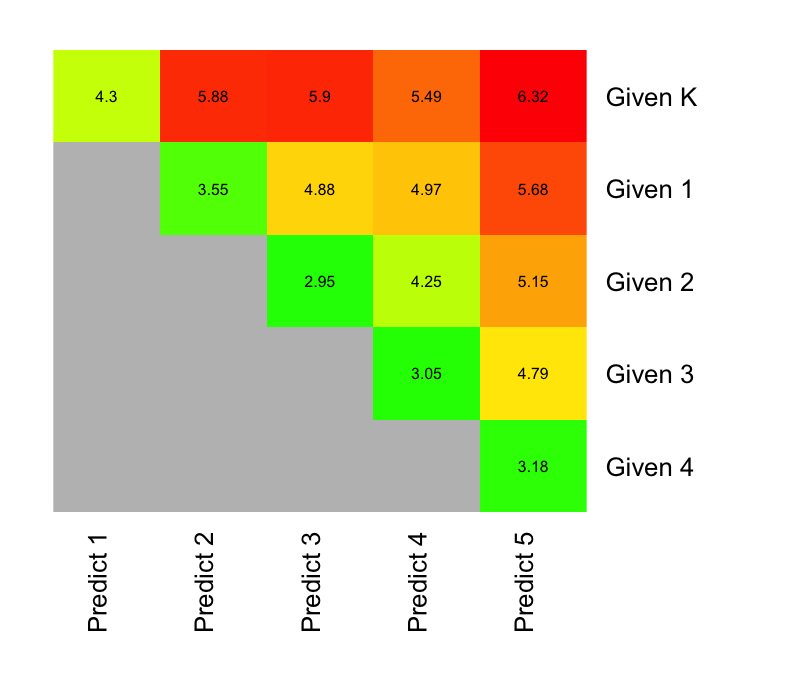
\includegraphics[width=3in,height=1.5in,clip,keepaspectratio]{lin_no_corr_error.png}
\\
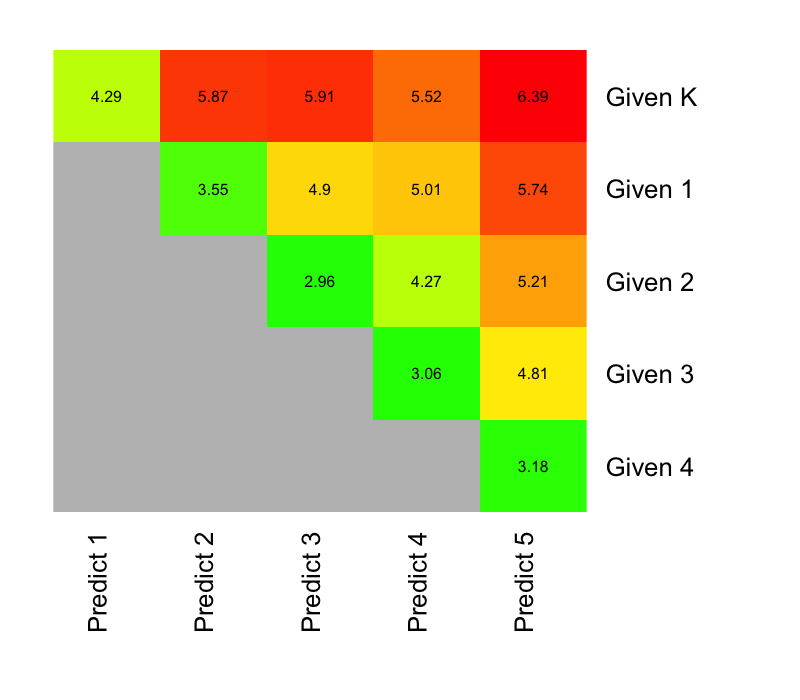
\includegraphics[width=3in,height=1.5in,clip,keepaspectratio]{no_change_error.png}
& \pbox{3.6cm}{\scriptsize Clockwise from Bottom Left:\\~~-Baseline model: Predict no change\\~~-Linear change with GMRF Prior\\~~-Exponential change with GMRF Prior\\~~-Linear change without GMRF Prior\\~~-Exponential change without GMRF Prior} \\
\end{tabular}
\caption{RMSE for each prediction task}
\label{tab:rmse_for_mm}
\end{table}

From these error matrices,we conclude:
\begin{itemize}
\item Cohort evolution models perform better than grade/time linear models (given their best test RMSE of \(\sim8.2\), and the worst task-specific test RMSE for the Markov models of 6.77).
\item In both cases, the GMRF prior actually decreases performance slightly. This will be addressed in more detail in the conclusion.
\item Overall, the model with no growth actually outperforms any of the growth models.
\end{itemize}

\section{Discussion}

At the outset of this paper, we presented our core hypothesis, namely that the census tracts' spatial structure could be exploited to improve the performance of predictive models. To exploit this spatial structure, we use the GMRF priors described by Lee \emph{et al} in \cite{lee2015carbayesst}, and tried applying this prior in two different classes of models: linear models, and markov chain models.
\subsection{Linear Models}

Overall, in our linear models, this prior provided some regularization. As seen in \ref{tab:model_1_results}, for unregularized models the training set RMSE decreased and the test set RMSE increased as model complexity increased. In contrast, using the GMRF prior, the training error was relatively unaffected by increasing model complexity.

That said, given the near equivalence of the experimental (GMRF prior) and control models for the feature set \({\beta_0, \beta_g, \beta_t}\), the added time-cost of model fitting (running the hamiltonian monte carlo sampler for several hours) is not justified. Instead, the simple linear model without the GMRF are sufficient- hence these experiments do not support the hypothesis that use of GMRF priors improves the models predictive performance. 

\subsection{Markov Chain Models}

In model 2 (markov chain growth models), we also got negative results for the hypothesis that spatial struture could be exploited to improve model performance. In these models, the GMRF-regularization actually decreased test set RMSE performance compared to unregularized models. We explain this observed result in terms of the bias-variance trade off. Specifically, this suggests that imposing spatial smoothness on cohort growth rates adds bias to the tract-level models, and does not return gains in the form of reduced variance. Hence, overall test set performance decreases as a result of this spatial regularization. Finally, we note that our Model experiments demonstrated essentially negligible test set performance gains using growth rate models compared to the simplest possible prediction: simply predicting no change (i.e. $r_k = 0$) for all tracts.

\subsection{Overall}

In both cases (linear and Markov chain models), our hypothesis was not supported. Importantly, one explanation for this is the granularity of the data (temporally, spatially, and in terms of the demographic specificity implied in the requirement to make grade-level predictions). While at this level of granularity exploiting spatial structure proved fruitless, we hypothesize this methodology may still prove effective for less granular tasks, since additional aggregation would smooth the data, and thus likely smooth the spatial distribution as well.

\section{Conclusions}

Overall, our study was premised on the hypothesis that spatial structure could be exploited to achieve significant gains in predictive performance. Unfortunately, this first premise proved to be incorrect. As such, if we were to continue working on this project, we would likely chose to consume side data and use it to expand the feature space. While we did not identify any features that seemed like reasonable evidence for incorporation in such a fine grained model (i.e. features that would be useful for predicting the number of second graders in a specific census tract, and ultimately a specific city block, for a specific year), perhaps additional research would reveal such a feature.

Additionally, we would also likely explore Hidden Markov Models instead of Markov Chains. Using HMMs, the added hidden layer could potentially usefully smooth the observed counts, and allow for better predictions.


% needed in second column of first page if using \IEEEpubid
%\IEEEpubidadjcol

% An example of a floating figure using the graphicx package.
% Note that \label must occur AFTER (or within) \caption.
% For figures, \caption should occur after the \includegraphics.
% Note that IEEEtran v1.7 and later has special internal code that
% is designed to preserve the operation of \label within \caption
% even when the captionsoff option is in effect. However, because
% of issues like this, it may be the safest practice to put all your
% \label just after \caption rather than within \caption{}.
%
% Reminder: the "draftcls" or "draftclsnofoot", not "draft", class
% option should be used if it is desired that the figures are to be
% displayed while in draft mode.
%
%\begin{figure}[!t]
%\centering
%\includegraphics[width=2.5in]{myfigure}
% where an .eps filename suffix will be assumed under latex, 
% and a .pdf suffix will be assumed for pdflatex; or what has been declared
% via \DeclareGraphicsExtensions.
%\caption{Simulation Results}
%\label{fig_sim}
%\end{figure}

% Note that IEEE typically puts floats only at the top, even when this
% results in a large percentage of a column being occupied by floats.


% An example of a double column floating figure using two subfigures.
% (The subfig.sty package must be loaded for this to work.)
% The subfigure \label commands are set within each subfloat command, the
% \label for the overall figure must come after \caption.
% \hfil must be used as a separator to get equal spacing.
% The subfigure.sty package works much the same way, except \subfigure is
% used instead of \subfloat.
%
%\begin{figure*}[!t]
%\centerline{\subfloat[Case I]\includegraphics[width=2.5in]{subfigcase1}%
%\label{fig_first_case}}
%\hfil
%\subfloat[Case II]{\includegraphics[width=2.5in]{subfigcase2}%
%\label{fig_second_case}}}
%\caption{Simulation results}
%\label{fig_sim}
%\end{figure*}
%
% Note that often IEEE papers with subfigures do not employ subfigure
% captions (using the optional argument to \subfloat), but instead will
% reference/describe all of them (a), (b), etc., within the main caption.


% An example of a floating table. Note that, for IEEE style tables, the 
% \caption command should come BEFORE the table. Table text will default to
% \footnotesize as IEEE normally uses this smaller font for tables.
% The \label must come after \caption as always.
%
%\begin{table}[!t]
%% increase table row spacing, adjust to taste
%\renewcommand{\arraystretch}{1.3}
% if using array.sty, it might be a good idea to tweak the value of
% \extrarowheight as needed to properly center the text within the cells
%\caption{An Example of a Table}
%\label{table_example}
%\centering
%% Some packages, such as MDW tools, offer better commands for making tables
%% than the plain LaTeX2e tabular which is used here.
%\begin{tabular}{|c||c|}
%\hline
%One & Two\\
%\hline
%Three & Four\\
%\hline
%\end{tabular}
%\end{table}


% Note that IEEE does not put floats in the very first column - or typically
% anywhere on the first page for that matter. Also, in-text middle ("here")
% positioning is not used. Most IEEE journals use top floats exclusively.
% Note that, LaTeX2e, unlike IEEE journals, places footnotes above bottom
% floats. This can be corrected via the \fnbelowfloat command of the
% stfloats package.

% if have a single appendix:
%\appendix[Proof of the Zonklar Equations]
% or
%\appendix  % for no appendix heading
% do not use \section anymore after \appendix, only \section*
% is possibly needed

% use appendices with more than one appendix
% then use \section to start each appendix
% you must declare a \section before using any
% \subsection or using \label (\appendices by itself
% starts a section numbered zero.)
%



% Can use something like this to put references on a page
% by themselves when using endfloat and the captionsoff option.
\ifCLASSOPTIONcaptionsoff
  \newpage
\fi



% trigger a \newpage just before the given reference
% number - used to balance the columns on the last page
% adjust value as needed - may need to be readjusted if
% the document is modified later
%\IEEEtriggeratref{8}
% The "triggered" command can be changed if desired:
%\IEEEtriggercmd{\enlargethispage{-5in}}

% references section

% can use a bibliography generated by BibTeX as a .bbl file
% BibTeX documentation can be easily obtained at:
% http://www.ctan.org/tex-archive/biblio/bibtex/contrib/doc/
% The IEEEtran BibTeX style support page is at:
% http://www.michaelshell.org/tex/ieeetran/bibtex/
\bibliographystyle{IEEEtran}
\bibliography{refs}
%
% <OR> manually copy in the resultant .bbl file
% set second argument of \begin to the number of references
% (used to reserve space for the reference number labels box)
%\begin{thebibliography}{1}

%\bibitem{IEEEhowto:kopka}
%H.~Kopka and P.~W. Daly, \emph{A Guide to \LaTeX}, 3rd~ed.\hskip 1em plus
%  0.5em minus 0.4em\relax Harlow, England: Addison-Wesley, 1999.

%\end{thebibliography}

% biography section
% 
% If you have an EPS/PDF photo (graphicx package needed) extra braces are
% needed around the contents of the optional argument to biography to prevent
% the LaTeX parser from getting confused when it sees the complicated
% \includegraphics command within an optional argument. (You could create
% your own custom macro containing the \includegraphics command to make things
% simpler here.)
%\begin{biography}[{\includegraphics[width=1in,height=1.25in,clip,keepaspectratio]{mshell}}]{Michael Shell}
% or if you just want to reserve a space for a photo:

%\begin{IEEEbiography}[{
\includegraphics[width=1in,height=1.25in,clip,keepaspectratio]{picture}}]{John Doe}
%\blindtext
%\end{IEEEbiography}

% You can push biographies down or up by placing
% a \vfill before or after them. The appropriate
% use of \vfill depends on what kind of text is
% on the last page and whether or not the columns
% are being equalized.

%\vfill

% Can be used to pull up biographies so that the bottom of the last one
% is flush with the other column.
%\enlargethispage{-5in}



% that's all folks
\end{document}


